\chapter{An Image-based Approach to Variational Path Synthesis of Linkages}\label{image_based_approach}

\section{Introduction}

\begin{figure*}[tbh]
\centering
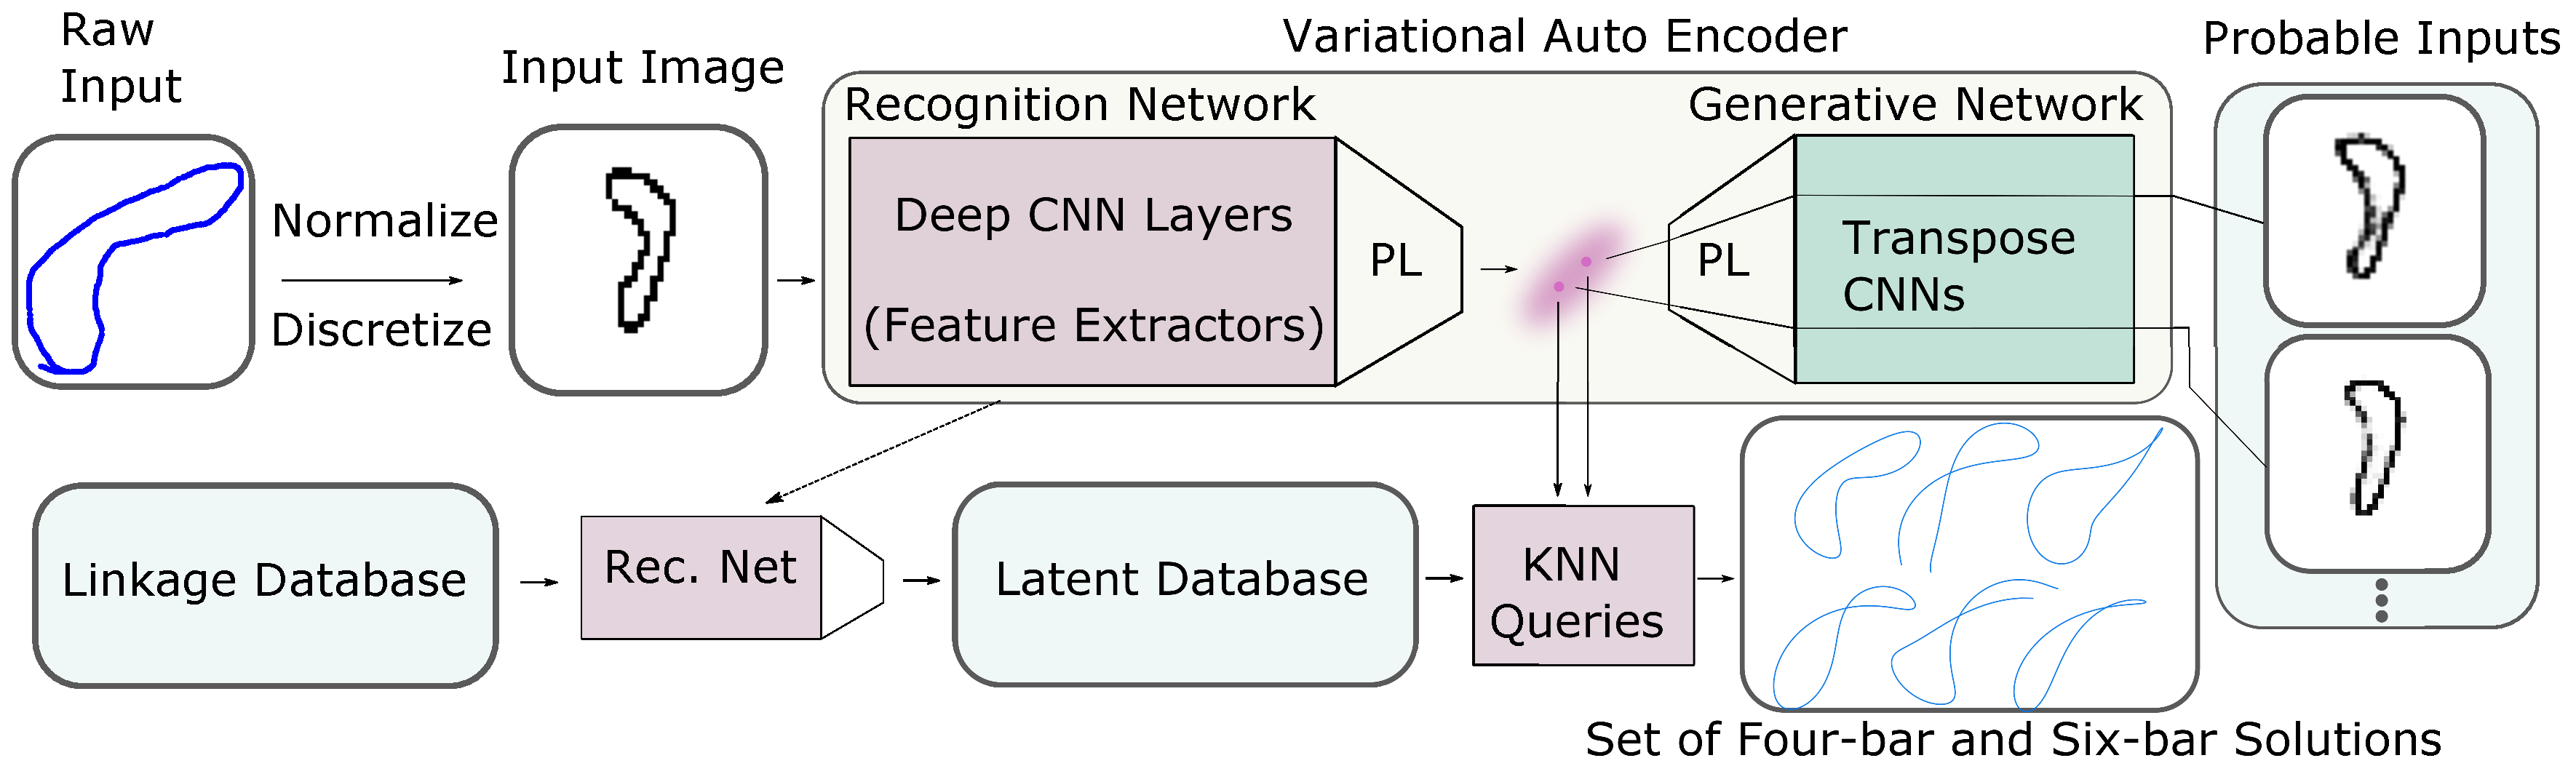
\includegraphics[width=0.9\textwidth]{idetc-20/figure/fig_overview.eps}
  \caption{Overview: Raw input is normalized and discretized into an image. This image is passed through the recognition network of a trained VAE which computes a probability distribution of latent features describing conducive variations of the raw input. Samples from this distribution are queried to find nearest neighbors in a dataset of four-bar and six-bar linkages. The linkages corresponding to the nearest neighbors have coupler curves similar to the conducive variations.}
\label{fig_contrasting_overview}
\end{figure*}
%%%%%%%%%%%%%%%%%%%%%%%%%%%%%%%%%%%%%%%%%%%%%%%%%%%%%%%%%%%%%%%%%%%%%%

This paper presents a novel approach that models the input path as a discrete probability distribution. This image-based novel representation allows us to employ the recent advances in computer vision and pattern recognition. The outcome is a probability distribution of conducive input possibilities, which efficiently enumerates alternative paths that highly correlate with the raw uncertain input. In addition, our deep generative model suppresses the infeasible portion of the input image and modifies it into a more conducive input, thereby proving feedback on the input. The approach is independent of the algebraic complexity of the coupler curve. Furthermore, deep learning techniques have an ability to learn arbitrarily complex spatial signals making it a scalable approach to learn all possible coupler curves.

Modeling the input path as a signal is a well-established idea in theoretical kinematics. Optimization-based techniques attempt to minimize an objective function and find mechanisms, which best approximates a curve generated by using the Fourier series~\cite{nolle1971}. Ullah and Kota\cite{ullah1997} have presented an invariant approach towards the representation and synthesis of closed-loop paths through shape optimization. They use a combination of global and local search methods for optimizing the Fourier Deviant function to compute the dimensions of planar four-bar linkages without an initial guess. Wu et al.\cite{wu2011} presented a method based on finite Fourier series for path generation of four-bar mechanisms.
In the case of motion generation, Li et al.\cite{li2016} have developed a Fourier descriptor-based approach for approximate motion generation.
Buskiewicz et al.\cite{Buskiewicz2009} used the curvature of the coupler curve for path synthesis using Genetic Algorithms.
Khan et al.\cite{khan2015} presented an approach where an artificial neural network is used for mapping between Fourier coefficients corresponding to a coupler path and corresponding linkage parameters.

In the above approaches, the input path is assumed as a one-dimensional input by parameterizing the input path as a function of time. It is advantageous in cases where the sequential nature of the path is important. Our proposed approach models the input as a 2D spatial signal which allows capturing non-sequential spatial correlations. In addition, classical approaches generally work for closed curves only, which leaves out a large possibility of solutions. In contrast, the proposed approach works for open as well as closed curves.  

In the classical path generation approach, a Fourier series approximation of input path is computed. Then, an optimization routine returns a linkage that closely approximates this task curve. This procedure narrows down the search space aiming to obtain a single accurate solution. On the contrary, our proposed approach takes in a raw, and often imprecise, input and computes a distribution of plausible inputs that capture the spatial correlations. This is enabled by first creating a standard form of all coupler curves and representing them as images, which are further fed to a deep generative machine learning model, called Variational Auto Encoder (VAE). The VAE generates sampling of new curves by using a probability distribution of latent features, which are learn by the model over time. Then, these plausible samples are used to find nearest neighbors in a database of four-bar and six-bar linkages. The result is a large set of solutions in contrast to a single optimal solution. Figure~\ref{fig_contrasting_overview} shows an overview of this approach. In the succeeding sections, we will present details of each of the components shown in the figure.

To the best of authors' knowledge, this is the first attempt to create 1) an image-based representation of input path which captures spatial correlations in the input path and provides a probabilistic estimate, 2) representation of coupler curves of different algebraic order in a unified way, and 3) Convolutional Neural Network-based state-of-the-art deep generative models that learn joint probability distribution of coupler curve images to generate variational inputs and provide the user feedback on the quality of input. 


The rest of this paper is organized as follows. Section~\ref{sec_image_representation} presents the details of image-based representation of coupler curves. Section~\ref{sec_deep_learning_vae_back} reviews the theory of convolutional neural networks. It also presents the motivation behind using the deep generative models along with the details of its architecture. Section~\ref{sec_vae_for_image} presents the applications of VAE for image-based path generation problem.

%%%%%%%%%%%%%%%%%%%%%%%%%%%%%%%%%%%%%%%%%%%%%%%%%%%%%%%%%%%%5

\section{Representing Coupler Curves as an Image}\label{sec_image_representation}
It is well-known that the coupler curves of linkage mechanisms are algebraic curves of degree 6 or more. In the case of the path generation problem, the task is to find a coupler curve (CC) that best fits a set of precision points. Thus, for all practical purposes, CC is represented as a discrete set of points given by,
\begin{equation*}
    \textrm{CC} = \{ x_i, y_i \}_{i=1}^N.
\end{equation*}

A common approach is to treat this sequence of points as a one dimensional temporal signal with parameter $t$ given by,  
\begin{equation*}
    \textrm{CC} = \{x(t), y(t)\}
\end{equation*}
This formulation allows for applying various signal processing techniques like Fourier Analysis. While this type of modeling has many advantages which are evident by the success in path generation, it fails to capture spatial correlations that are not implicit in temporal correlations.

The proposed image-based representation allows us to capture those correlations in exchange for losing temporal correlations between the input sequences.
However, it can be argued that the the ordering is embedded in the spatial distribution of pixels since unlike typical computer vision applications, such as facial recognition, which have a true 2D set of pixels for images, a curve is fundamentally a one-dimensional entity only. In addition, if the task does not need a specific ordering of points, the image based approach allows for capturing all possible input orders in a unified way.

\subsection{Standard Form and Pixel Mapping}
In this paper, an image represents a probabilistic coupler curve, where the intensity of a pixel represents likelihood of containing a coupler curve point. First, each coupler curve is normalized with respect to scale, position and orientation.

\paragraph{Normalization}

First, the path is subtracted by the mean $(\bar{x}, \bar{y})$. The translated curve is divided by the root mean squared variance in Cartesian $X$- and $Y$-directions.
To make the representation invariant to orientation, the curve is rotated such that its principal component axes are aligned with the coordinate axes. Figure~\ref{fig_curve_normalization} depicts the normalization procedure for two couple paths.

\begin{figure}
\centering
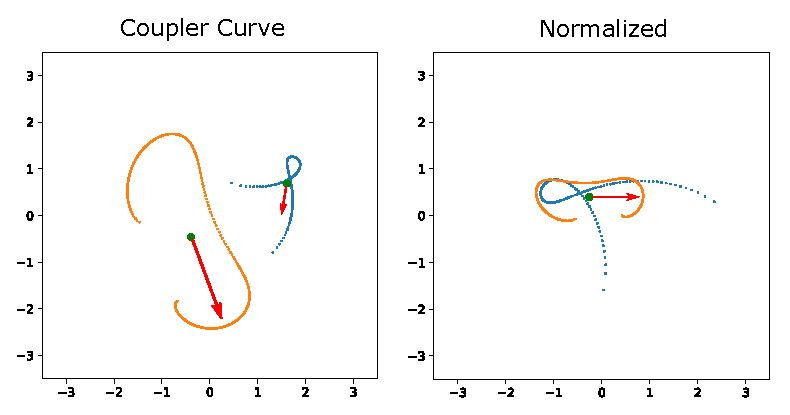
\includegraphics[width=250pt]{idetc-20/figure/fig_curve_normalization.eps}
  \caption{Each curve is normalized for position, scale and orientation.}
\label{fig_curve_normalization}
\end{figure}

The principal component axes are eigenvectors of the covariance matrix $C$ of a coupler path comprising of $m$ two-dimensional points $\{x_j, y_j\}_{j=1}^{m}$, where $C$ is given by,
\begin{eqnarray}
  C = \left[
\begin{array}{cc}
  C_{xx}  & C_{xy}  \\
  C_{yx}  & C_{yy}
\end{array}
\right],  \textrm{where}\\
C_{xx} = \frac {1}{m} \sum_{i=1}^{m}(x_i - \bar{x})(x_i - \bar{x}) ,\\
C_{yy} = \frac {1}{m} \sum_{i=1}^{m}(y_i - \bar{y})(y_i - \bar{y}) ,\\
C_{xy} = C_{yx} = \frac {1}{m} \sum_{i=1}^{m}(x_i - \bar{x})(y_i - \bar{y}).
\end{eqnarray}

\paragraph{Discretization}
The normalized planar curve is now discretized into a 2D image. The two-dimensional Cartesian space is linearly discretized into $S-1$ partitions along each axis, where $S$ corresponds to a side of the image.
The partitions along $X$ axis is done as follows:
$x$ coordinates that lie between $-\infty$ to $-X_{lim}$ are binned into a the first partition. The next partition includes $x$ ranging from $(-X_{lim}, -X_{lim} + X_{step}]$, and so on up to the last partition $(X_{lim}, +\infty)$. Here, $X_{lim}$ and $X_{step}$ are discretization parameters, which control the range and resolution respectively. Figure~\ref{fig_curve_discretization} depicts the discretization of a normalized curve. It can be noted that the extreme coordinates play an important role in deciding resolution and range of pixels. 


\begin{figure}
\centering
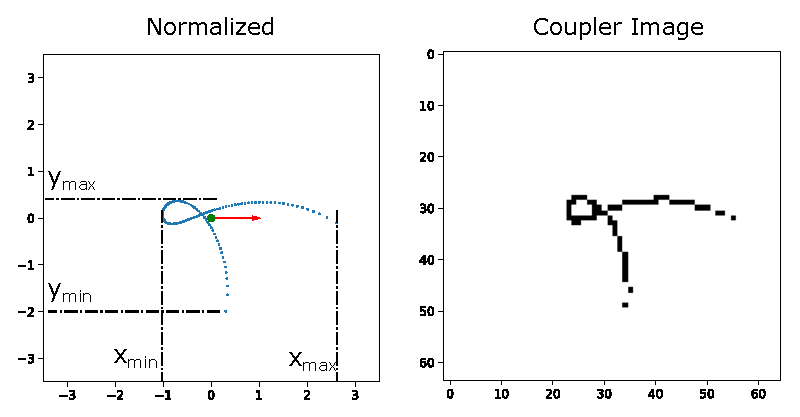
\includegraphics[width=250pt]{idetc-20/figure/fig_curve_discretization.eps}
  \caption{The extreme coordinates ($x_{min}, x_{max}, y_{min}, y_{max}$) of a normalized coupler curve are shown. If a point lies in Cartesian span of pixel, it is given 1.0 probability.}
\label{fig_curve_discretization}
\end{figure}


\begin{figure}
\centering
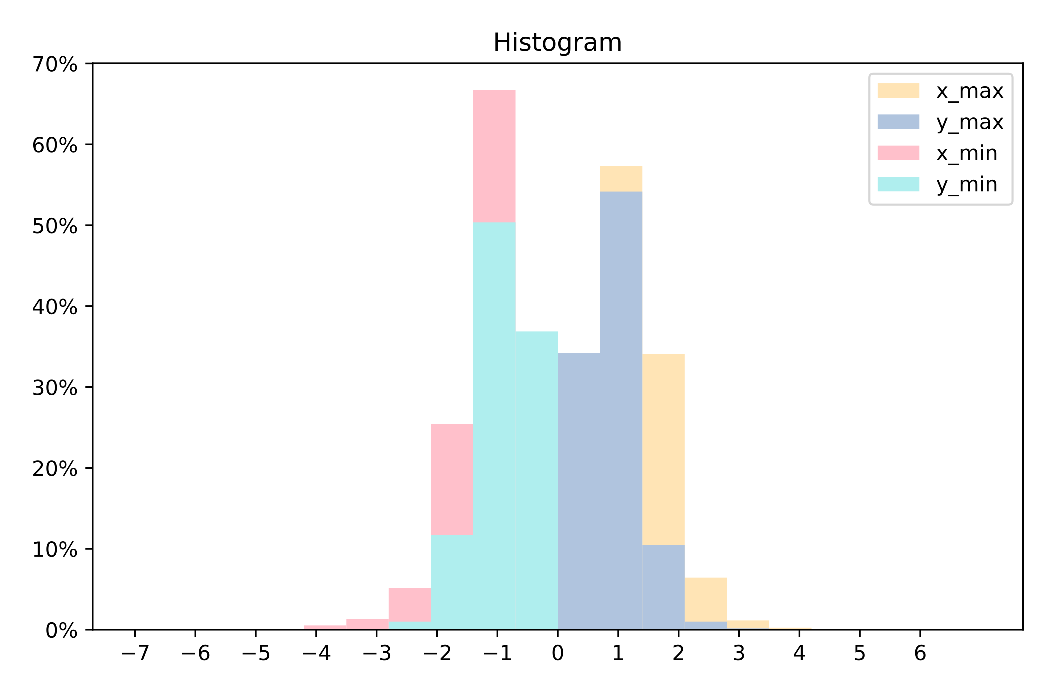
\includegraphics[width=250pt]{idetc-20/figure/fig_histogram.eps}
  \caption{A histogram of extreme coordinates ($x_{min}, x_{max}, y_{min}, y_{max}$) of coupler curves. It can be seen that less than $1\%$ of the normalized coupler curves have a point with an absolute coordinate larger than 3.5 units.}
\label{fig_histogram}
\end{figure}




To estimate $X_{lim}$, a statistical study is conducted on a dataset of 6,818 linkages comprising of four-bar (2,188), Stephenson I (2,754) and Stephenson III (1,876) six-bar linkages. The coupler curve for each linkage is stored as a sequence of points sampled per one degree change in crank angle. The number of points in coupler curves are different for different mechanisms. Figure~\ref{fig_histogram} shows the histogram of extreme coordinates corresponding to the normalized coupler curves from the database. It can be seen that more than $99\%$ of linkages are contained by a square with a side 7 and center at the origin. Thus, $X_{lim}$ is set as $7/2 = 3.5$. 
For an image with ($S\times S$) pixels, $X_{step}$ is given by,
\begin{equation*}
   X_{step} = \frac{2X_{lim}}{S - 1}.
\end{equation*}
Here, each pixel of an image represents a probability of containing at least one point of the coupler curve.
In this paper, we choose $S = 64$, which provides sufficient resolution to capture the variation in coupler curves. 
Figure~\ref{fig_curve_discretization} depicts the discretization of a normalized coupler curve into an image.
It should be noted that the discretization process causes some loss of information. However, in many cases, the input is inherently vague. Thus, it acts as a buffer and prevents the further process from over-emphasizing the numerical precision. One can also notice that image-based representation removes the order of points in the curve. However, it grants spatial correlations between neighboring points, which helps in capturing interesting spatial patterns. In section~\ref{sec_deep_learning_vae_back}, we review some of the techniques that are used to learn and recognize such spatial patterns.



\subsection{CNN-VAE Architecture for Image Representation of Coupler Curves}

VAE~\cite{Kingma2014AutoEncodingVB} is a neural network architecture, which learns to approximate the true distribution of an observed data $X$.
In this work, VAE is trained to learn the distribution of coupler curves in the form of images. Thus, here $X$ is an $S\times S$ image.
Figure~\ref{fig_conv_vae} shows a general architecture of VAE.
In this architecture, the Recognition Model encodes the data into the probability distribution of latent variables, while the Generative Model is responsible for generating new data or reproducing trained data.
In this figure, the recognition model consists of multiple stacks convolutional, ReLU and Max Pooling layers. At the end of the final stack, a fully connected layer outputs two vectors $\mu$ and $\sigma$, respectively. These two vectors correspond to parameters of multivariate Gaussian distribution.
The generative model takes a sample vector $z$ from the Gaussian distribution and outputs an image $\hat{X}$ given by,
\begin{eqnarray}
pr(z) = \mathcal{N}(0, 1)\label{pz},\\
  \hat{X} = G(z; \theta_g)\label{eq_G},
\end{eqnarray}
where $\theta_g$ are weight parameters of the neural network that acts as the generative model.
The variable $z$ is called the latent variable, which contains salient information of the observed image $X$.
We would like to infer salient attributes $z$ based on observed $X$, which can be expressed by conditional probability $pr(z|X)$
\begin{equation}
pr(z|X) = \frac{pr(X|z)pr(z)}{pr(X)},
\end{equation}
where the abbreviation $pr(A)$ represents probability of variable $A$.
Unfortunately, computing probability of $X$ (i.e., $pr(X)$) is usually intractable because it involves computing the integral $\int
pr(X|z)pr(z)dz.$
However, we can apply variational inference~\cite{blei2017variational} to estimate the joint probability distribution $pr(z|X)$.
We approximate $pr(z|X)$ by a distribution $q(z|X)$, which we define such that it can be computed by a neural network $Q$.
\begin{eqnarray}\label{eq_Q}
\mu, \sigma = Q(X; \theta_e),\\
  q(z|X) = \mathcal{N}(\mu, \sigma)
\end{eqnarray}
Here, $\mathcal{N}(\mu, \sigma)$ is a multivariate Gaussian distribution function with mean $\mu$ and variance $\sigma$.
Now, we want to find parameters of Recognition Model $Q(X)$ that predict the distribution $q(z|X)$ such that it is very similar to $pr(z|X)$. Then, we can use it to perform approximate inference of the intractable distribution.

The objective is to find parameters $\theta_g, \theta_e $ of $G(z)$ and $Q(X)$ respectively such that our model generates samples as close as true observed distribution and distribution $q(z|X)$ is as close as true distribution $p(z)$.
This is achieved by training the neural network models for maximizing the Expectation Lower Bound (ELBo) of the marginal likelihood, which is given by,
\begin{equation}\label{elbo_loss}
  L_{ELBo}^{(X^i)} = \mathbb{E}_{Q(z|X^{i}; \theta_e)}(\log(p(X^{i}|z))) - D_{KL}(Q(z|X^{i}; \theta_e)||p(z))  \\
\end{equation}
Here, the first term on RHS represents reconstruction likelihood and the second term is called Kullback-Leibler divergence (KL divergence)~\cite{kullback1951} which ensures that our learned distribution $Q(z|X;\theta_e)$ is similar to the true prior distribution $p(z)$.
Since we assume that $p(z)$ is a Gaussian distribution, the lower bound of marginal likelihood becomes,
\begin{equation}
  L_{ELBo}^{(X^i)} = - L_{\text{Cross Entropy}}(\hat{X}, X) - (\sum_i^{k} {\sigma_i}^2 + {\mu_i}^2 - \log(\sigma_i) - 1) \\
\end{equation}
where $L_{\text{Cross Entropy}}$ between $\hat{X}$ and $X$ is given by,
\begin{equation}
    L_{\text{Cross Entropy}} = -X\log(\hat{X}) + (X - 1)\log(1 -\hat{X})
\end{equation}

The training objective is given by,
\begin{equation}
 \argminA_{\theta_e, \theta_g} ( - L_{ELBo}^{(X^i)})
\end{equation}

For further details on VAE; please see \cite{Kingma2014AutoEncodingVB}.
Once, entire VAE is trained, the recognition model and generative model can be used separately or together depending upon the application.

\section{VAE for Coupler Images}\label{sec_vae_for_image}
This section presents the architecture and training details of the VAE used for the coupler image recognition and generation task. 
The training goal is to maximize the variational lower bound $L_{ELBo}$ given in Eq.~\req{elbo_loss} by changing the weights of recognition and generative models via stochastic gradient descent.
Maximizing the variational lower bound increases the likelihood of a given image to be the image of an actual coupler curve. Higher the likelihood, the more accurate the pixel intensities would get. 

\subsection{Architecture}
The input to the encoder is a $64\times64$ image. This input is fed to three stacks of convolutional-MaxPooling layers. The output of the convolutional layer is first passed through ReLU activation before it can be max pooled. Max pooling layer passes the highest activation in the filter window to the next layer. The hyper-parameters for each layer are given in Table~\ref{tab_encoder_paras}. After three such layers, the output is flattened into a single vector, which then is connected to a single fully connected layer which outputs two vectors representing $\mu$ and $\log\sigma$ of 50 dimensions each. Vector $z$ is obtained by sampling a multivariate Gaussian distribution with mean $\mu$ and standard deviation $\sigma$. This vector is passed to the generative model as an input.

\begin{figure*}[t]
\centering
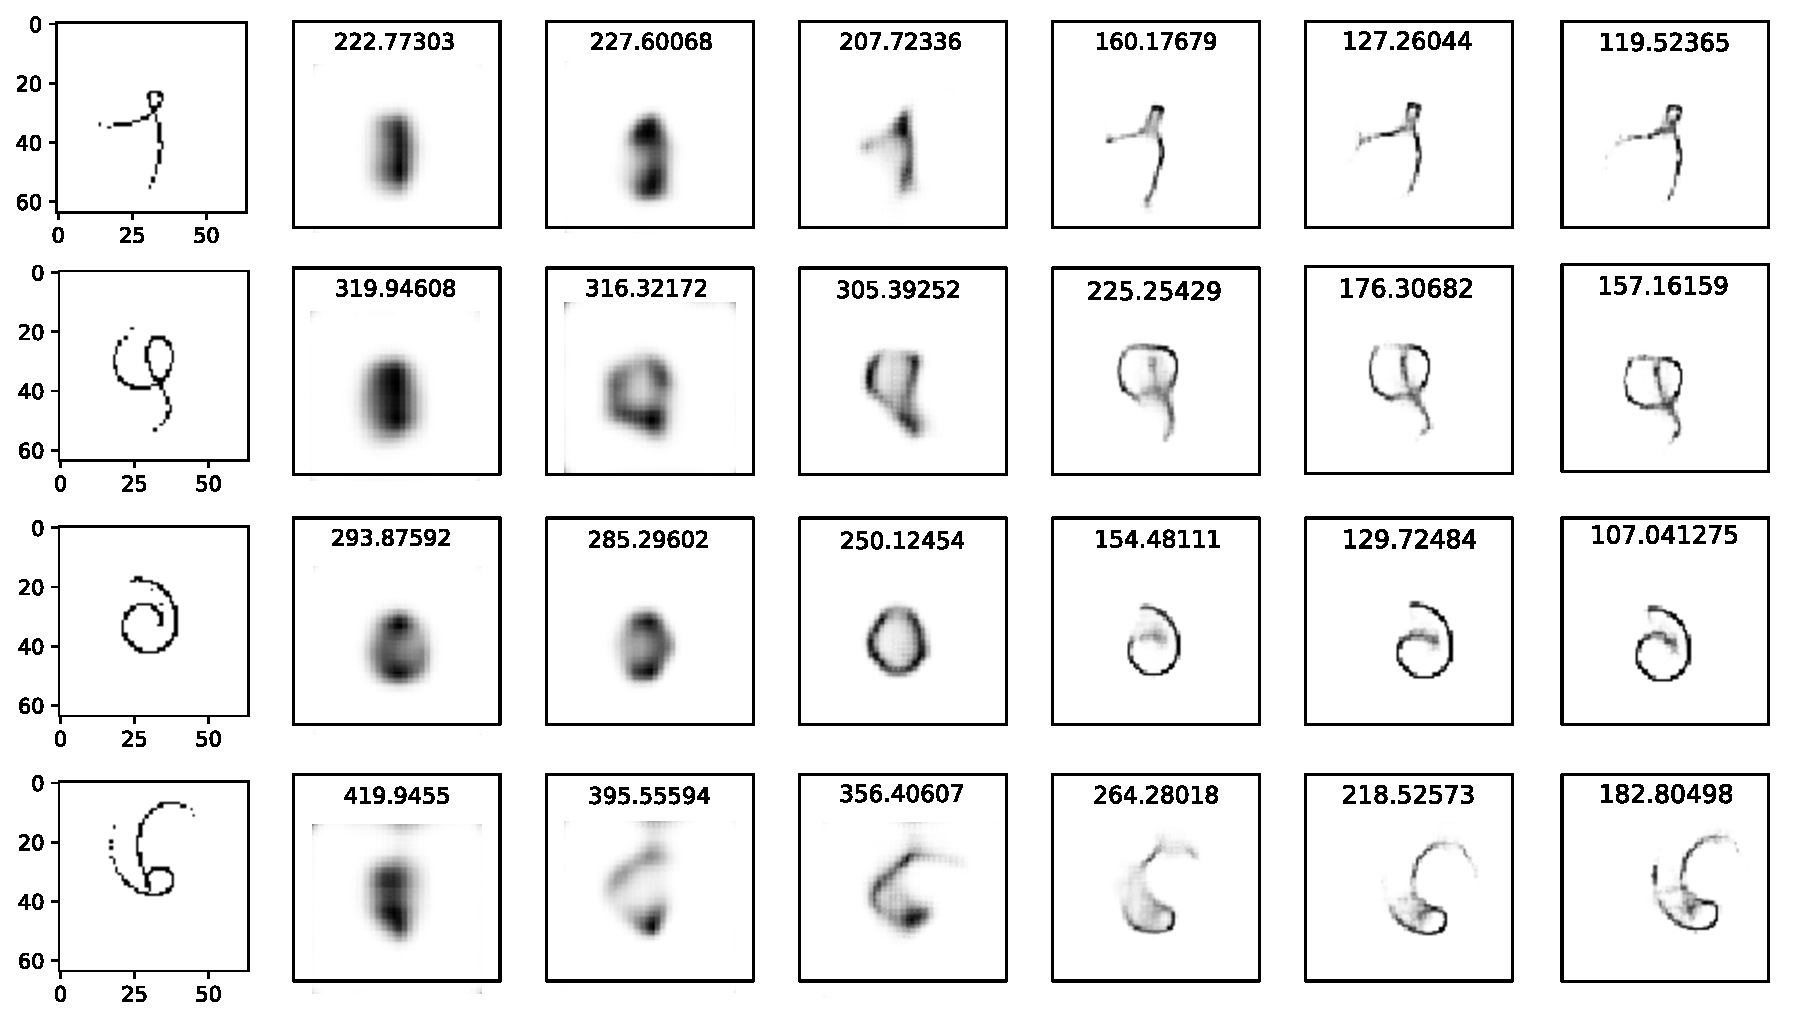
\includegraphics[width=0.75\textwidth]{idetc-20/figure/training_testing.eps}
  \caption{The training progress is reflected in the reconstruction quality of test coupler curve images. The corresponding variational lower bound $L_{ElBo}^{X^i}$ is displayed above each reconstructed image. It can be seen that the probability assignment by VAE for each pixel improves over the training.}
\label{fig_training_reconstructions}
\end{figure*}

\begin{table*}
  \caption{Recognition Network Architecture}
\centering
\label{tab_encoder_paras}
\begin{tabular}{cccccc}
\hline
  Layer & Filter Count & Filter Size & Stride & Output Shape & Activation\\
\hline
  Convolution 1 & 32 & (11, 11) & (1,1) & (64, 64, 32) & ReLU \\
  Max Pooling 1 & - & (2,2) & (2,2) & (32, 32, 32) & -  \\
  Convolution 2 & 64 & (5, 5) & (1,1) & (32, 32, 32) & ReLU   \\
  Max Pooling 2 & - & (2,2) & (2,2) & (16, 16, 64) & - \\
  Convolution 3 & 128 & (3, 3) & (1,1) & (16, 16, 128) & ReLU   \\
  Max Pooling 3 & - & (2,2) & (2,2) & (8, 8, 128) & - \\
  Flatten 1 & - & - & - & 8192 & - \\
  Fully Connected & - & - & - & 100 & - \\
  Split & - & - & - & (2, 50) & (-, exponential) \\ \hline 
\end{tabular}
\end{table*}



The generative model architecture is composed of transpose-convolution layers to finally output a tensor similar to that of image. The architecture and hyper-parameters are given in Table~\ref{tab_decoder_paras}.

\begin{table*}
  \caption{Generative Network Architecture}
\centering
\label{tab_decoder_paras}
\begin{tabular}{cccccc}
\hline
  Layer & Filter Count & Filter Size & Stride & Output Shape & Activation\\
\hline
  Fully Connected & - & - & - & 1024 & ReLU \\
  Reshape & - & - & - & (8, 8, 16) & - \\
  Transpose Convolution 1 & 128 & (3, 3) & (2,2) & (16, 16, 128) & ReLU   \\
  Transpose Convolution 2 & 64 & (5, 5) & (2,2) & (32, 32, 64) & ReLU   \\
  Transpose Convolution 3 & 32 & (11, 11) & (2,2) & (64, 64, 32) & ReLU   \\
  Transpose Convolution 3 & 1 & (3, 3) & (1,1) & (64, 64, 1) & Sigmoid   \\
\hline
\end{tabular}
\end{table*}

\subsection{Training}
Figure~\ref{fig_training_reconstructions} shows improvement in reconstructions of coupler image samples from the test set as the training progresses. It can be seen that the pixels with a higher probability of containing a coupler point are assigned a higher probability and vice versa. 
Once the network is trained sufficiently, the encoder learns to capture spatial correlations and returns a probability distribution in latent feature space. Each sample from this distribution has a high probability of being a valid coupler image. 
This feature is used to obtain feasible representations of raw input and is demonstrated in Section~\ref{subsec_raw_recogn_rec}. 

\subsection{Raw Input Recognition and Reconstruction}\label{subsec_raw_recogn_rec}
Raw user input is defined as an image with a different distribution of pixel intensities than the ones the VAE has learned while training. 
If such an input image is fed to VAE, the recognition network tries to find the learned patterns in the input. The patterns with high correlation with learned patterns will receive a high score that will be passed through max-pooling layers and eventually reflect in the obtained latent distribution. If samples from that distribution are passed through the generative model, it will produce coupler curve-like images that share similar spatial attributes.
Figure~\ref{fig_prob_shift_effect} shows examples where VAE takes in raw inputs and computes feasible inputs that are used for downstream tasks for path generation. It can be seen that VAE shifts the probability assignments on the pixels of the raw input. Figure~\ref{fig_prob_shift_effect} highlights this effect on various raw inputs. This is used to provide feedback on the user input.    
Figure~\ref{fig_two_inputs} depicts the outcome of VAE construction for two different inputs. The input shown on the top can be closely approximated by a four-bar mechanism, whereas the other input is highly unlikely for a four-bar or six-bar to interpolate. Since the VAE is trained on coupler curves of four-bar and six-bar linkages, it can reconstruct the original input with high accuracy. On the other hand, second input is highly modified by VAE to change it into a more conducive input. The difference between the modification done by VAE is reflected in percentage change in histogram of pixel intensities. For the first image, almost $70\%$ of the pixels retain their original $100\%$ intensity, whereas that number is a mere $17\%$ for the second input. 

\begin{figure*}
\centering
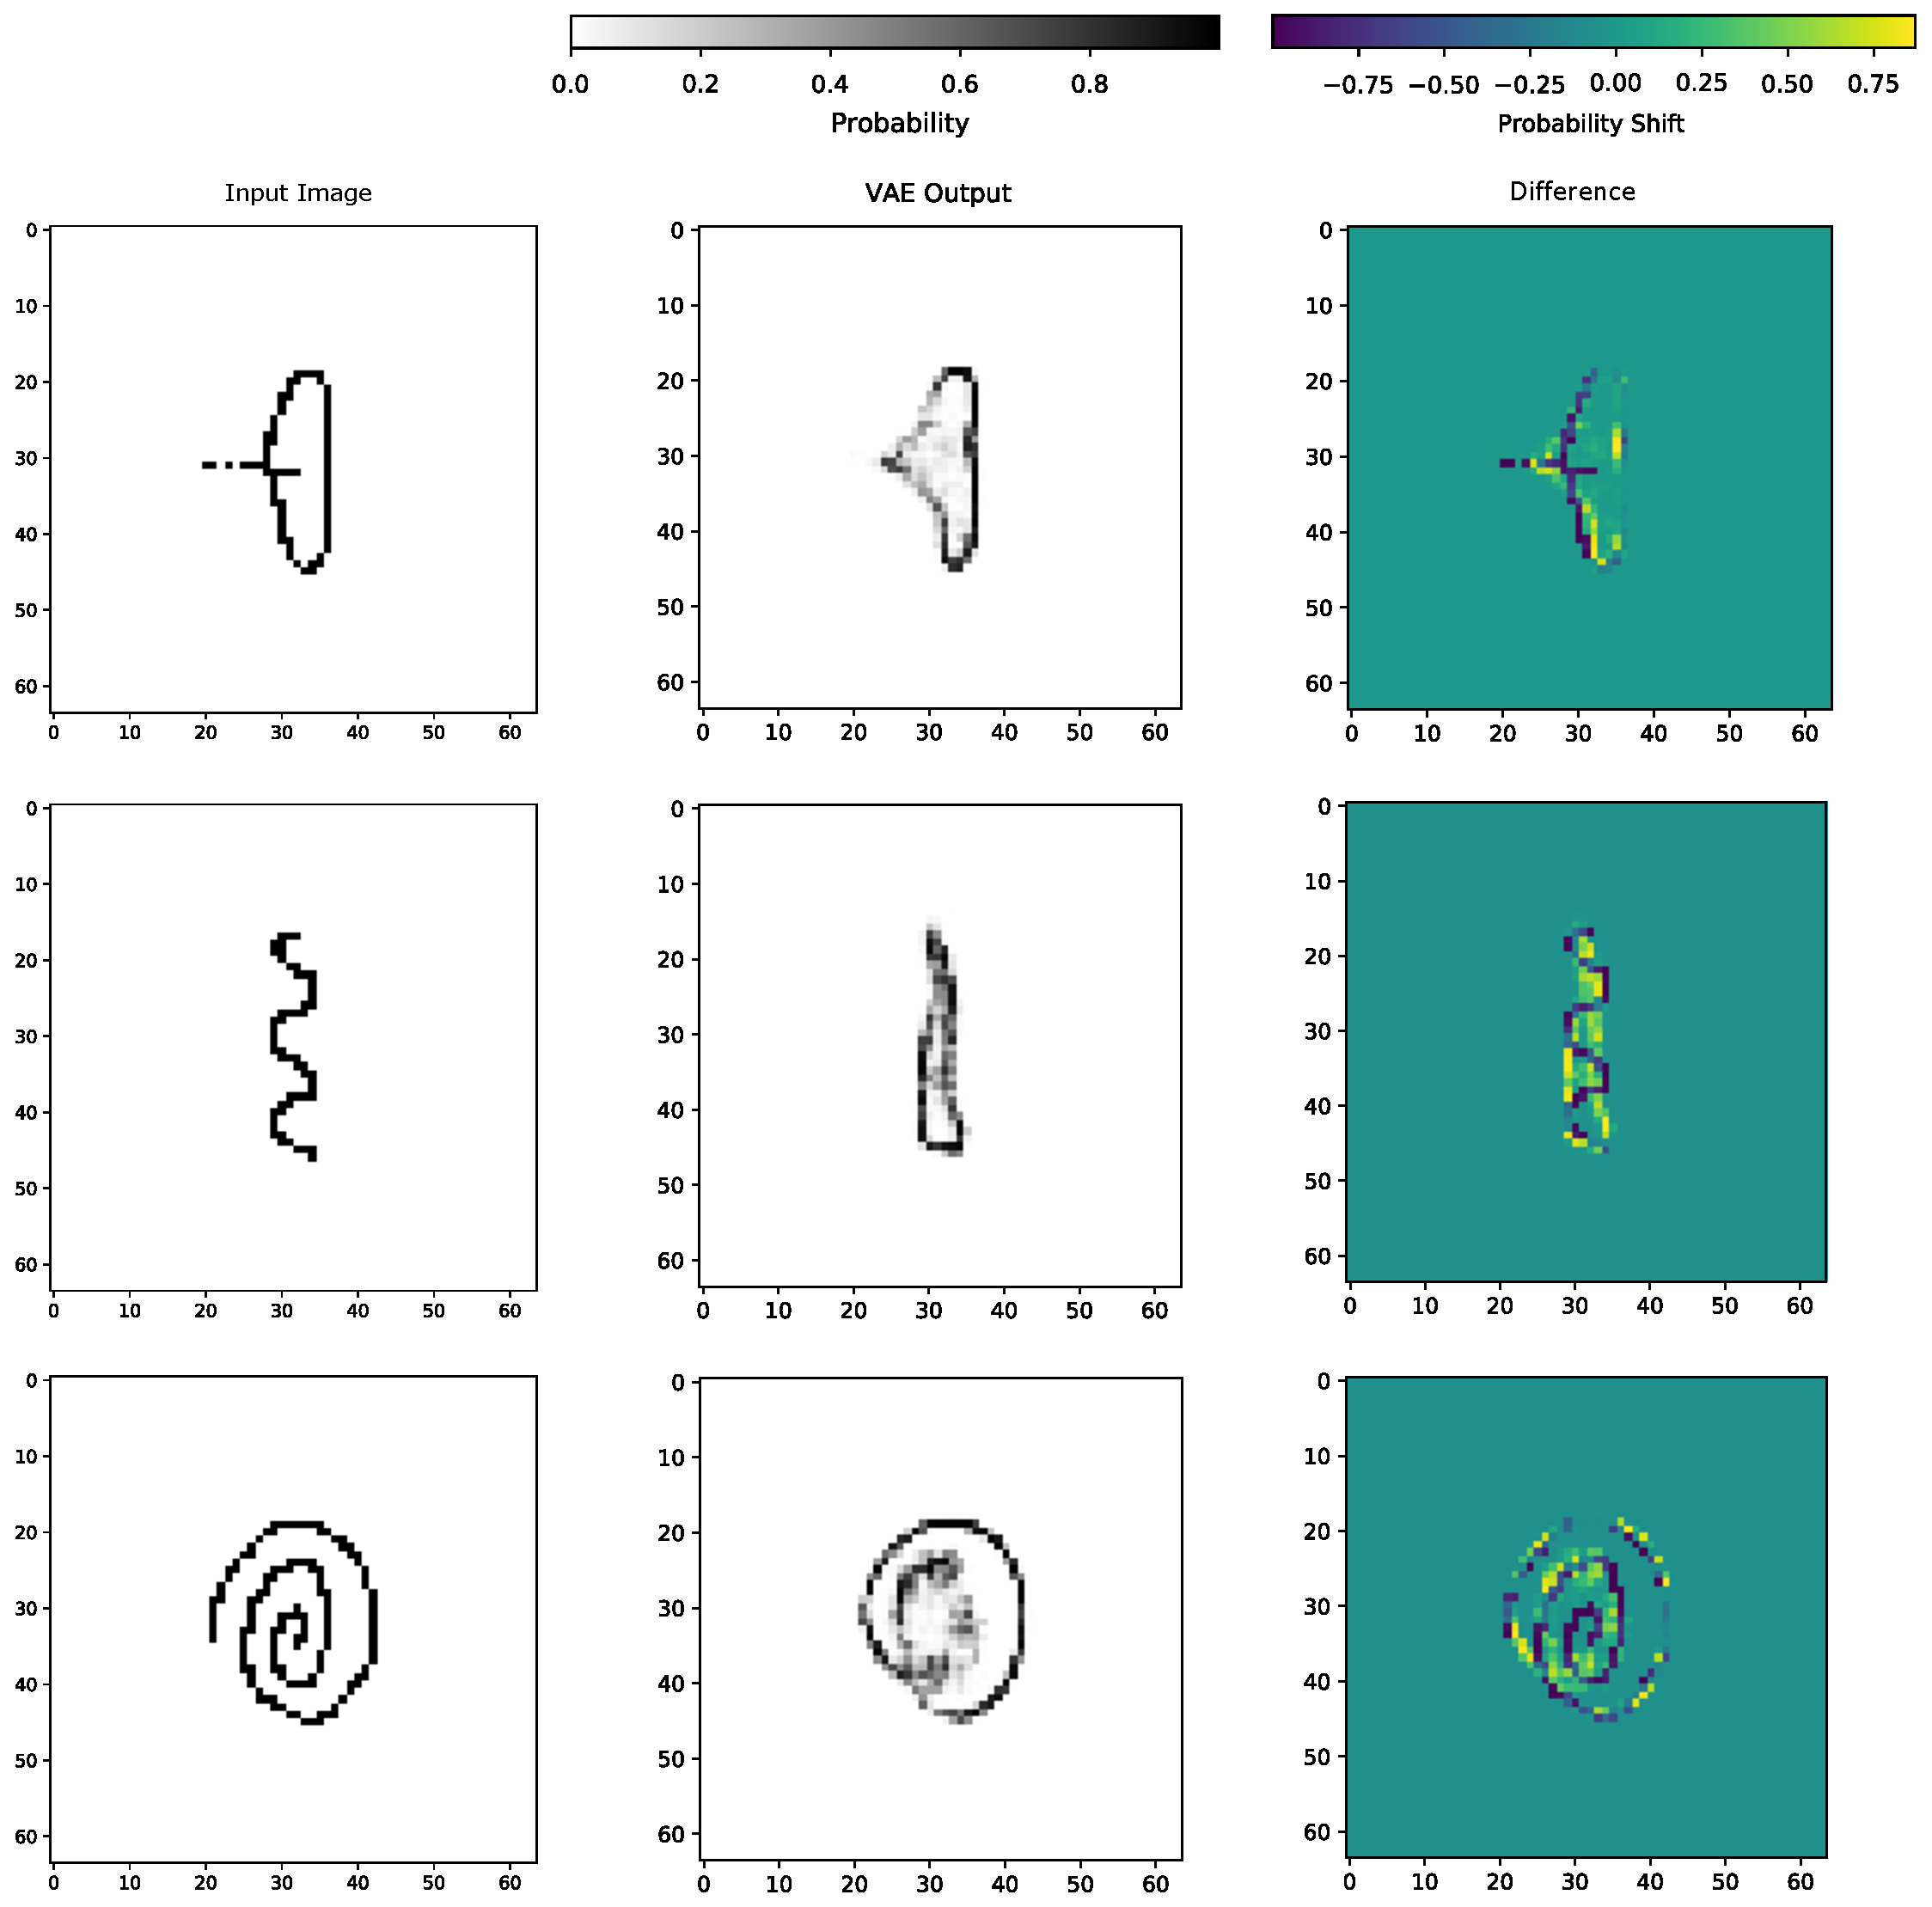
\includegraphics[width=0.75\textwidth]{idetc-20/figure/probability_shift.eps}
  \caption{Raw input image is passed through VAE which provides a feasible input image. The shift in the probabilities is highlighted in the rightmost images. The shift shown in dark indicates that the portion of raw input is highly unlikely for linkage from the dataset to interpolate. This provides visual and intuitive feedback to the user on the input.}
\label{fig_prob_shift_effect}
\end{figure*}

\begin{figure*}
\centering
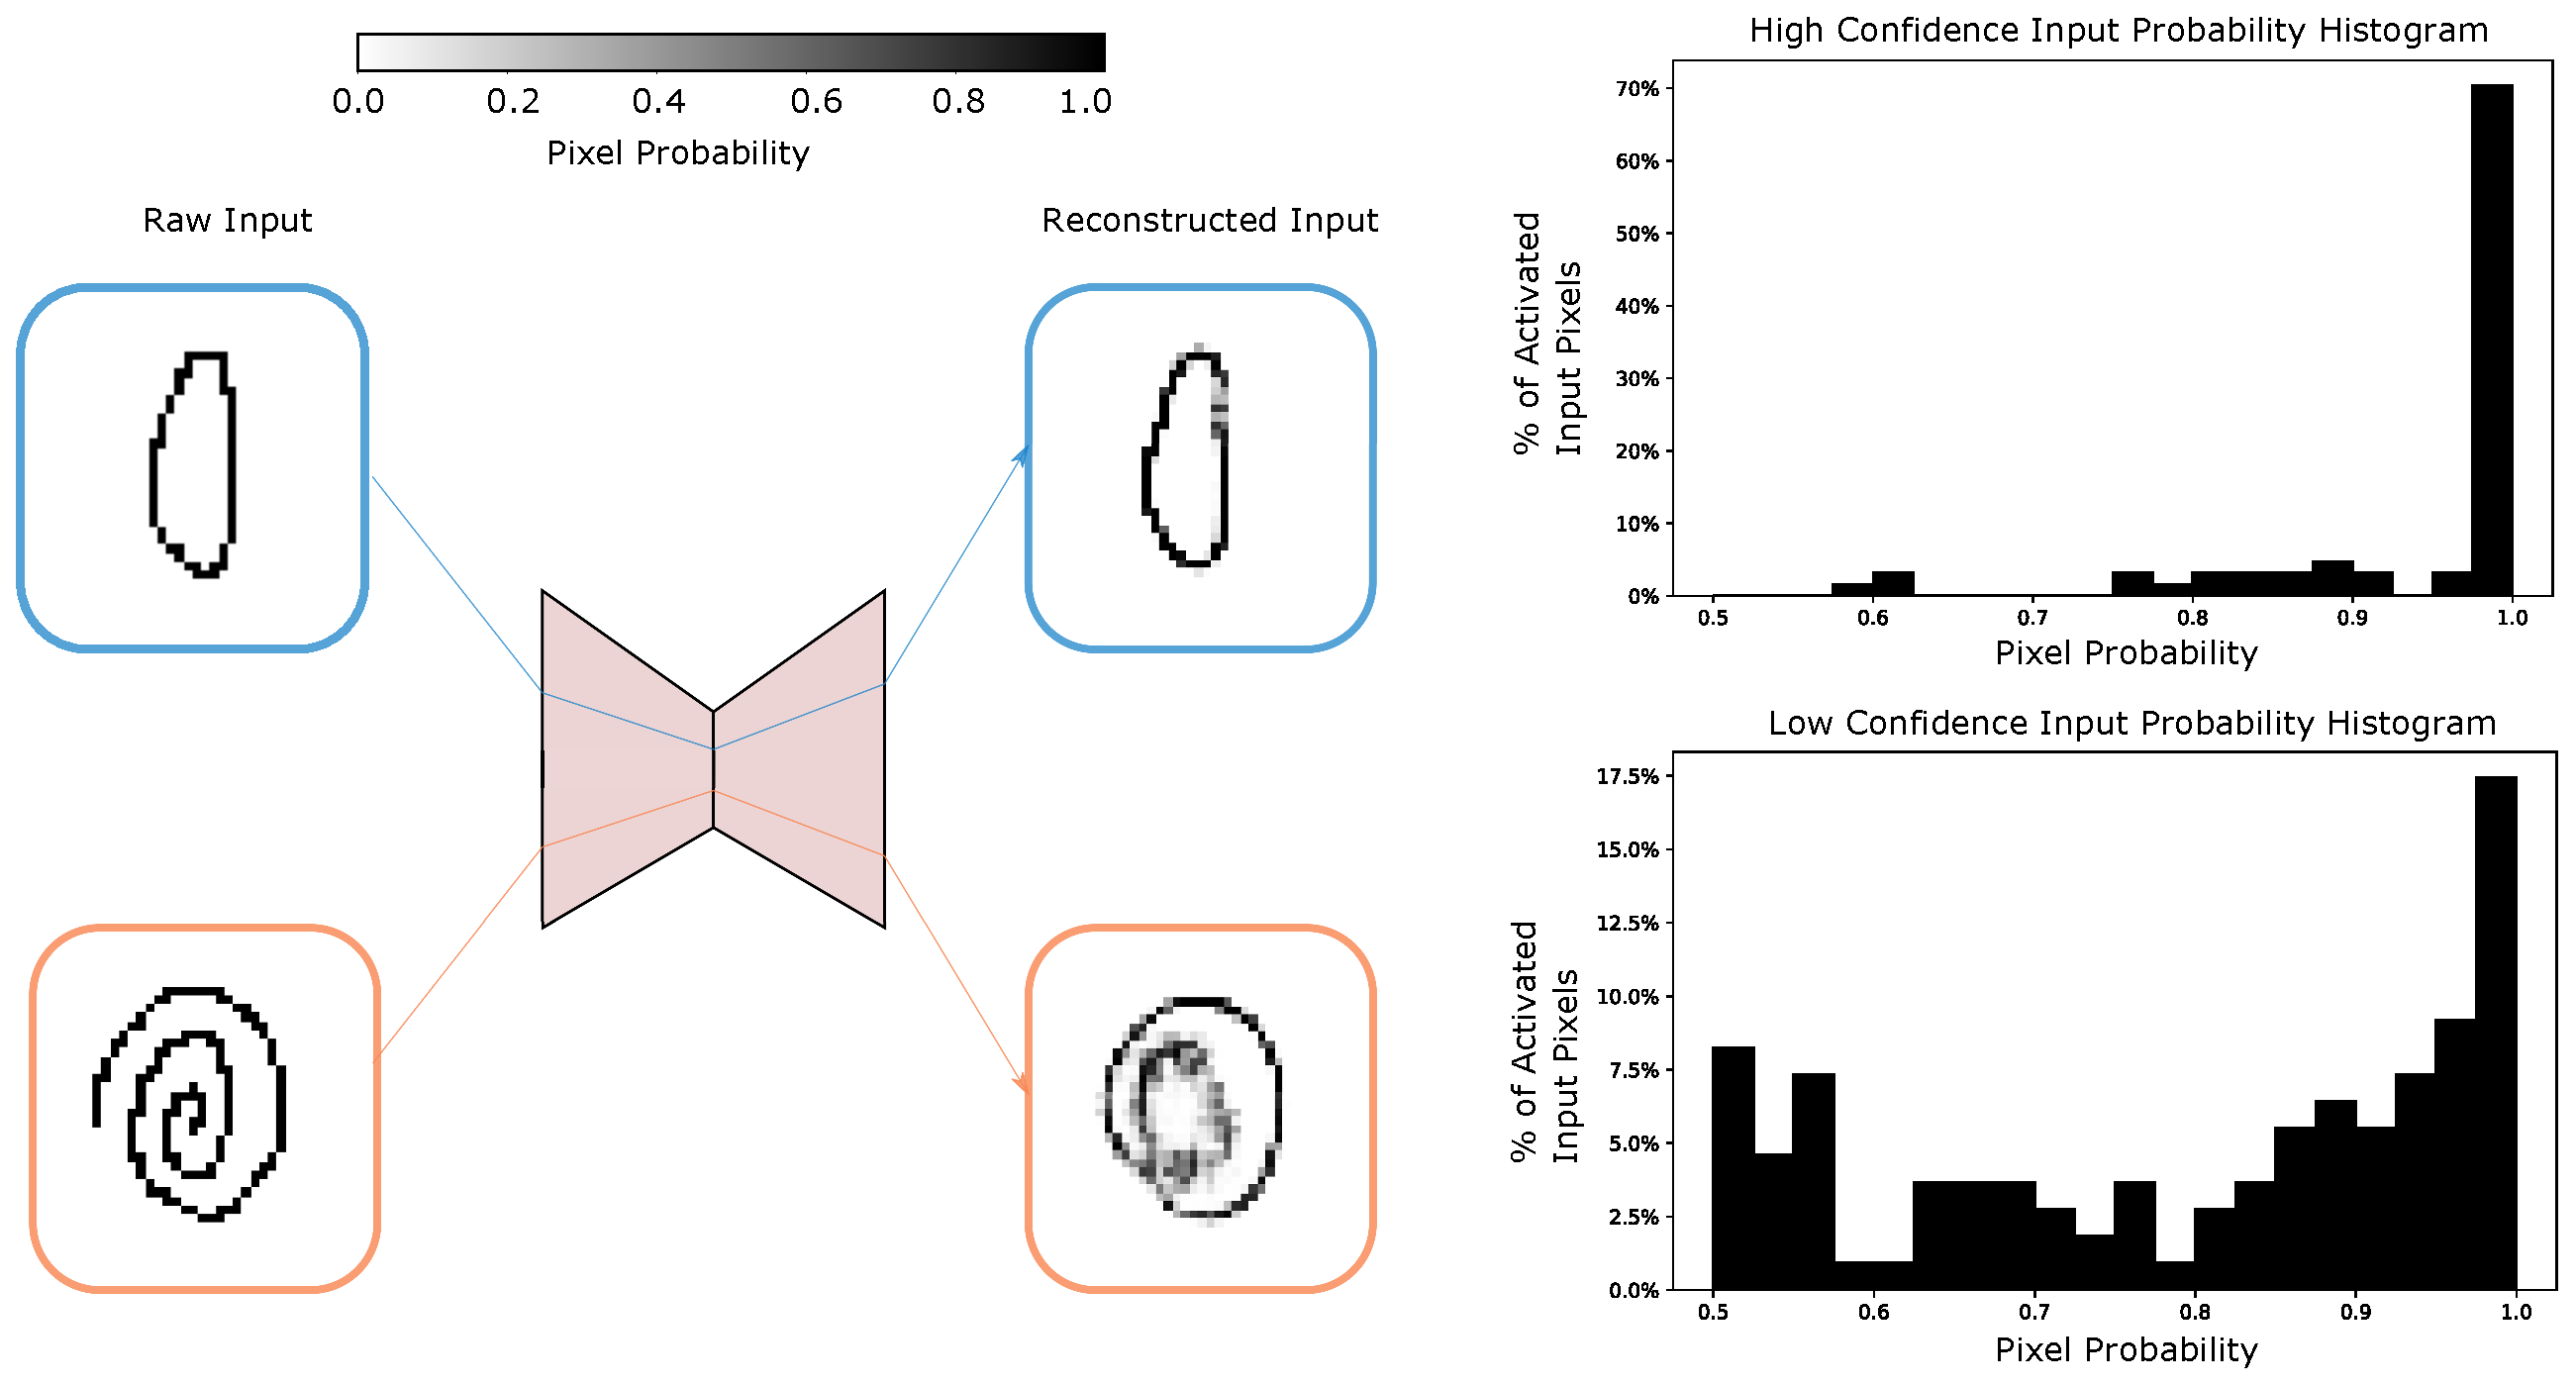
\includegraphics[width=0.75\textwidth]{idetc-20/figure/high_low_confidence_feedback_new.eps}
  \caption{The raw input on the top is close to the true distribution of coupler curves, thus VAE retains almost $70\%$ of the highest intensities as depicted by the histogram on the top. For the second input, VAE overrides user assignments on the input pixels by a large number. This is due to highly spiral nature of the input. It can be also seen in Fig~\ref{fig_prob_shift_effect} that inner portion of the input is highly penalized. }
\label{fig_two_inputs}
\end{figure*}

\begin{figure*}
\centering
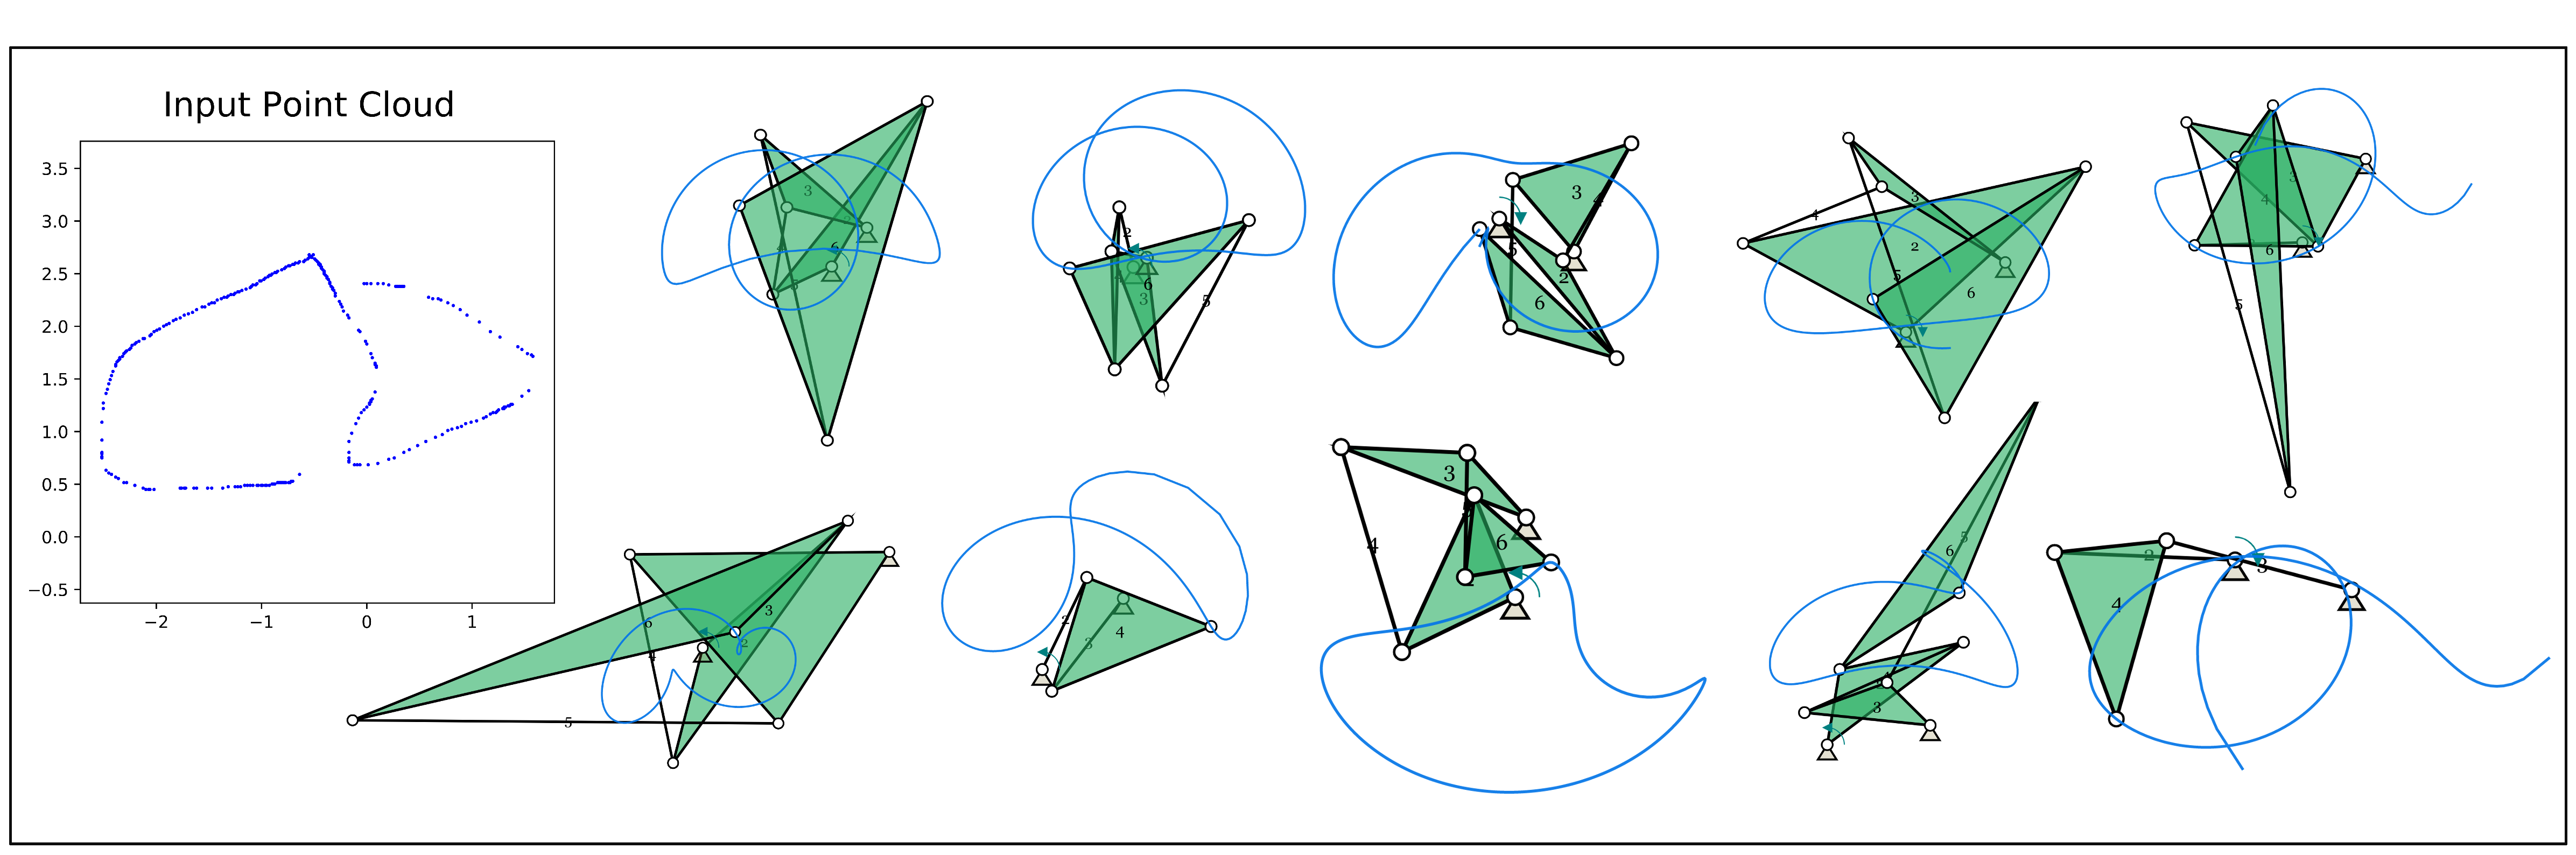
\includegraphics[width=0.85\textwidth]{idetc-20/figure/fig_knn_latent.eps}
  \caption{The linkages corresponding to the K nearest neighbor in latent space for the given raw input are depicted. It can be seen that the linkages exhibit a wide variety in terms of their coupler path; thereby capturing input uncertainty.}
\label{fig_knn_latent}
\end{figure*}
\subsection{Nearest Latent Neighbors for Variational Path Synthesis}

In Section~\ref{subsec_raw_recogn_rec}, it was shown that the recognition network captures the spatial correlations that highly correspond to that of coupler curve images. To take advantage of this fact, the database is remapped into a 50-dimensional space where each mechanism is represented by the latent vector obtained using the recognition model. At the time of synthesis, raw input is passed through the recognition model to find a distribution of possible latent vectors. K-Nearest neighbors to the mean of this distribution are returned as potential solutions. Figure~\ref{fig_knn_latent} presents some of the solutions obtained for the nearest neighbor query on raw user input. 



